\documentclass[12pt]{ctexart}
\usepackage{amsfonts,amssymb}
\usepackage{float}
\usepackage{graphicx}
\usepackage{amsmath}
\usepackage{listings}
\usepackage{geometry}
\usepackage[usenames,dvipsnames]{xcolor}
\usepackage{setspace}
\geometry{a4paper}
\geometry{top=2cm} 
\geometry{bottom=2cm}
\geometry{left=0.5cm}
\geometry{right=1cm}

\title{数学实践~项目作业}
\author{凌子恒 \\ 信息与计算科学 3200102551}

\begin{document}

\maketitle

\subsection*{实现细节及解释}

画图见 plot.py,主函数为 main.cpp。

\subsubsection*{矩阵}

迭代法的复杂度只和矩阵非 $0$ 元素个数有关,且待求解的矩阵为稀疏矩阵,因此在 matrix.h 中实现了稀疏矩阵乘法和迭代。迭代参数 $w$ 固定为 $\dfrac{2}{3}$。

\subsubsection*{多重网格}

实现在 multigrid.h 中。由于不同维度的多重网格处理不同,分别实现每个维度的情况。

reset size 将 $\phi$ 通过 restriction 和 interpolation 调整为指定大小。

restriction 使用的是 $2^D$ 个超立方体的平均值,interpolation 直接将一个超立方体分为 $2^D$ 个值相等的超立方体。这两个函数都暴露在类外,便于 reset size 调用。

multigrid 类的构造函数传入一个获得矩阵的函数、一个获得等式右边项的函数和初始估计以及各种参数。构造后自动求解,可以调用:

\begin{itemize}
	\item get residual 获得余项(误差)
	\item get times 获得迭代次数(便于调整参数)
	\item get result 获得结果
\end{itemize}

\subsubsection*{有限体积法}

设 $N=\dfrac{1}{h}$,用一个向量 $\phi$ 表示 $\phi$ 在每个大小为 $h^D$ 的超立方体中的函数平均值。其中,左下角为 $(x_1,x_2,\cdots,x_D)$ 的超立方体平均值为 $\phi_{\sum\limits_{i=1}^D x_iN^{D-i}}$。

注意到对于每个 $s$,通过枚举求和符号中的 $j$ 可以计算出矩阵 $A$ 和列向量 $b$。由于系数计算较为复杂,且需要递归地处理,在类内实现 equations 类处理。

系数计算完成后,可以使用多重网格法求解 $A\phi^{(s)}=b$。

多重网格法需要对每个 $s$ 不同的 $N$ 计算 $A_N,b_N$,其中许多计算是重复的。因此可以考虑记忆化,如在 $lhs pool[g]$ 存储 $N=2^g$ 时的 $A_N$,需要时直接传参而不需要重复计算。

由于多重网格法得到 $A$ 后并不会进行修改,因此只需要传 pool 一个元素的常量引用即可,可以减少复制,提高效率。

特别的,对于时间无关的情况,$A$ 对每个 $s$ 甚至每轮迭代都是相同的,每个 $N$ 都只需要计算一次。

由于需要计算的数据量较大,为提高效率,代码复用率较低。

\subsection*{结果分析}

由于代码用时极长,不建议完整复现。

\subsubsection*{1.1 Traveling sinusoidal waves}

\title{$2$ 维}

调用函数 task 1,实现类为 FVMOL 1。

输出文件和图片开头为 $1.1$。由于图片相似,只选 $N=512$ 的进行展示:

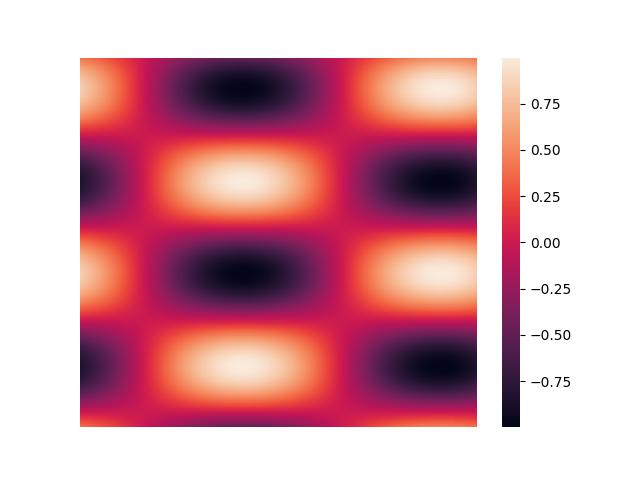
\includegraphics[scale=0.8]{1.1(N=512).jpg}

\begin{tabular}{c|c|c|c|c}
	$N$   &  $\Vert E\Vert _2$    &  $\Vert E\Vert_\infty$  &  $p_2$&  $p_\infty$  \\
	\hline
	$64$   &  $2.83\times 10^{-5}$    &  $8.12\times 10^{-5}$  & $4.0$ & $4.0$ \\
	$128$   &  $1.80\times 10^{-6}$    &  $5.08\times 10^{-6}$  & $4.0$  & $4.0$ \\
	$256$   &  $1.14\times 10^{-7}$    &  $3.17\times 10^{-7}$  & $4.0$ & $4.0$ \\
	$512$   &  $7.19\times 10^{-9}$    &  $1.98\times 10^{-8}$  &   & \\
\end{tabular}

计算收敛阶为 $p=4$。

\title{$3$ 维}

调用函数 task 1 3d,实现类为 FVMOL 1 3d。

输出文件开头为 $1.1.2$,未作图。

\begin{tabular}{c|c|c|c|c}
	$N$   &  $\Vert E\Vert _2$    &  $\Vert E\Vert_\infty$  &  $p_2$&  $p_\infty$  \\
	\hline
	$16$   &  $2.32\times 10^{-1}$    &  $6.73\times 10^{-1}$  & $0.9$ & $1.0$ \\
	$32$   &  $1.24\times 10^{-1}$    &  $3.45\times 10^{-1}$  & $1.0$  & $1.0$ \\
	$64$   &  $6.30\times 10^{-2}$    &  $1.78\times 10^{-1}$  & $1.0$ & $1.0$ \\
	$128$   &  $3.16\times 10^{-2}$    &  $8.97\times 10^{-2}$  &   & \\
\end{tabular}

计算收敛阶为 $p=1$。

\subsubsection*{1.2}

调用函数 task 2,实现类为 FVMOL 2。

输出文件和图片开头为 $1.2$。由于图片相似,只选 $N=512$ 的进行展示:

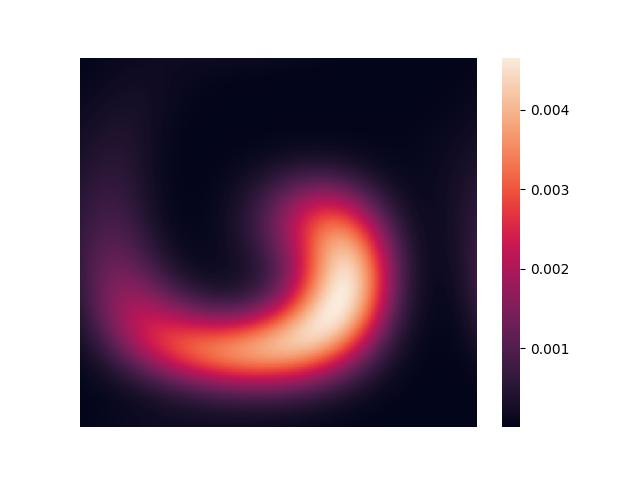
\includegraphics[scale=0.8]{1.2(N=512).jpg}

\begin{tabular}{c|c|c|c|c}
	$N$   &  $\Vert E\Vert _2$    &  $\Vert E\Vert_\infty$  &  $p_2$&  $p_\infty$  \\
	\hline
	$64$   &  $8.97\times 10^{-5}$    &  $2.96\times 10^{-4}$  & $1.0$ & $1.1$ \\
	$128$   &  $3.97\times 10^{-5}$    &  $1.22\times 10^{-1}$  & $1.0$  & $1.0$ \\
	$256$   &  $1.32\times 10^{-2}$    &  $4.01\times 10^{-2}$  & & \\
\end{tabular}

计算收敛阶为 $p=1$。

\subsubsection*{1.3}

调用函数 task 3,未完成。

\end{document}
